\chapter{Locally-linear pictorial structures}\label{sec:llps}
\section{Introduction}
\out{
Human pose estimation from single, 2D images holds great potential to assist in 
a wide range of applications---semantic indexing of images and videos, action 
recognition, activity analysis, and human computer interaction, to name a few.
However, human pose estimation ``in the wild'' is an extremely challenging 
problem.  It shares all of the difficulties of object detection, such as 
confounding background clutter, lighting, viewpoint, and scale, in addition to
significant difficulties unique to human poses.  }


In this chapter, we focus explicitly on the multi-modal aspect of the 2D pose 
estimation problem.  As discussed in~\secref{perceptual}, there is an enormous 
variation in foreground and background color and texture, and even given 
viewpoint and pose, the shape of body parts is highly variable due to clothing, 
relative scale variations, and articulation (causing foreshortening, 
self-occlusion and physically different body contours).

\begin{figure}[t!]
\centering
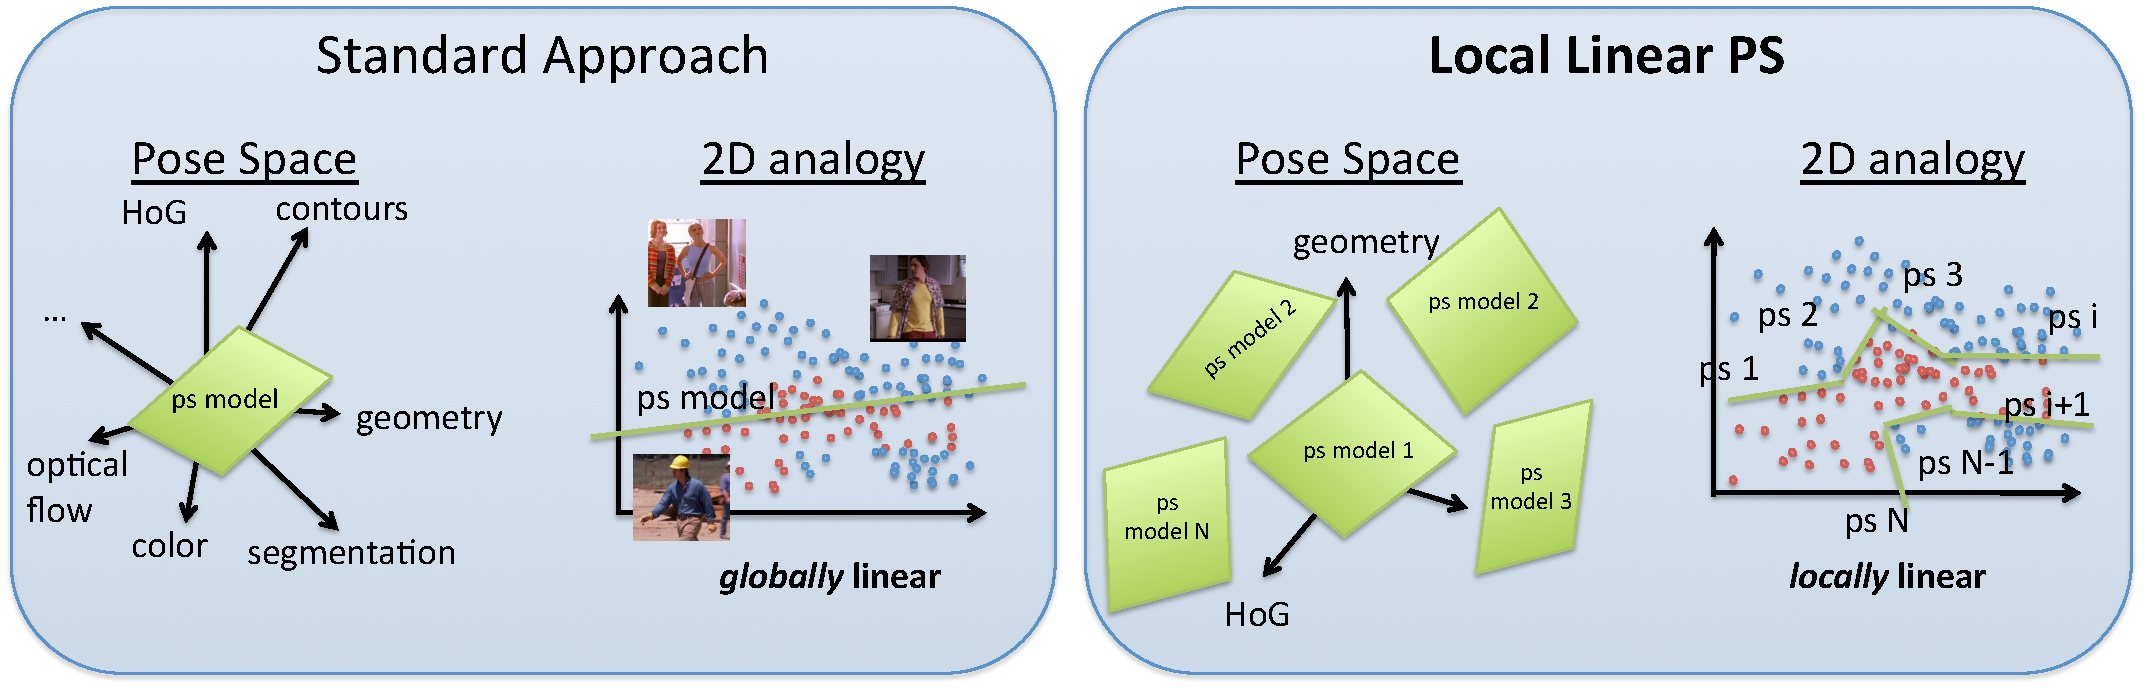
\includegraphics[width=0.99\linewidth]{figs/llps-overview.pdf}
\caption[LLPS overview.]{\label{fig:overview} \textbf{Left:} Most pictorial 
structures researchers have put effort into better and larger feature spaces, 
in which they fit one linear model.  The feature computation is expensive, and 
we still fail at capturing the many appearance modes in real data.  
\textbf{Right:} We take a different approach.  Rather than introduce more and 
more features in hopes of high-dimensional linear separability, we model the 
non-linearities in simpler, lower dimensional feature spaces, using a 
collection of {\em locally} linear models.}
\end{figure}


Most models developed for this use {\em only a single, linear model}---\eg, 
\citet{devacrf,eichner09,andriluka09,ddtran} and the models developed 
in~\secref{CPS} and~\secref{stretchable}.
Such models make it very difficult to capture the part variations discussed.  
Instead, most researchers focus attention on improving features in hopes that a 
better feature space will make a linear model discriminate correct poses from 
incorrect ones well.  

Recently, especially the past two years, there have been an explosion of work 
focused on increasing the number of modes in pose models, with much success.  
This line of work can generally be described as instantiations of a {\em family 
} of compositional, hierarchical pose models.  The family of models can be 
parametrized by the number of part levels (\eg, {\em \{ wrist, lower arm, full 
arm, half-body, full body \}} are example parts in a 5-level hierarchy) and the 
number of modes captured per part.  Part modes can capture different poses 
(\eg, elbow crooked, lower arm sideways) and appearance (\eg, thin arm, baggy 
pants).


 \begin{table}[tb]
\begin{center}
{\tiny
\begin{tabular}{| r | c | c |c | c | c | c | c |}
\hline
model &	atomic unit & part levels & training obj. & \# global modes	& \# part modes	& graph type & latent modes?	\\
\hline
basic ps	& limbs	& 1 &	parsing	& 1	& 1	& tree & no \\
\cite{wang2008multiple} & limbs & 1 &	parsing &	3	& 1	& tree &	no \\
\cite{everingham2011} &	limbs &	1 &	parsing &	16 & 4* &	tree &	yes \\
\cite{deva2011} &	joints & 1	& detection &	1 &	4 to 6 & tree	& yes \\
\cite{wang2011} & limbs & 4	& parsing	& 1 &	5 to 20 & cyclic & no \\
\cite{sun2011} & limbs	& 4	&	parsing	& 1	& 4	& tree & yes \\
\cite{ramanan-faces} &	joints &	1	& detection &	18	& 1** &	tree	& yes \\
\cite{batra2012} & joints	& 4	&	detection &	9 &	4 to 6 & cyclic &	no \\
\cite{tianexploring} & limbs & 3 & detection	& 5 &	5 to 15 &	tree & yes \\
\hline
OURS & joints & 2 & both & 32 & 1 & tree & no \\
\hline
\end{tabular}



}
\caption[Coarse-to-fine cascade progression analysis.]{Coarse-to-fine cascade 
progression analysis. We show the progression of state spaces in the cascade, 
as well as reduction in the state space at each level (measuring efficiency), 
and in the last column, how many arm hypotheses remain closely matched, 
considering the closest match to groundtruth remaining from the unpruned 
hypotheses (measuring accuracy). }
\label{tab:rel-work-ps} \end{center}
\end{table}



\mypar{Our approach:} In this chapter, we propose a model of human pose that 
defines a mode {\em per training example}, to capture a local neighborhood of
pose {\em and } appearance.  This results in hundreds or thousands of modes in 
contrast to the 20 or fewer used by recent work. This gives us the ability to 
precisely model pose and appearance using a linear, structured model for each 
local neighborhood.  Because of this defining characteristic, we call our model 
\LLPSlong~(\LLPS).

We define the extent of each neighborhood in terms of radii in appearance and 
pose, which decompose at a part level.  As a result, the training example space 
is well covered, and we have overlap between modes.  This allows us to heavily 
share training data and gives us a smoothly varying representation of the space 
of 2D human poses.

Using our explicit formulation of locality, no latent modes need to estimated, 
and no decisions made as to quantization degree and mode placement.  We propose 
a simple convex max-margin learning objective to fit parameters of our model.  
We show our model is competitive with state-of-the-art approaches from this 
year, while employing only very simple features. Further, inference is cheap 
and heavily parallelizable, taking only a few seconds per image.


\section{Related work}
Here we take a particular perspective on some of the popular recent 
approaches~\citet{devacrf,eichner09,sapp2010cascades,sapp2011,andriluka09,ddtran}.  
Recently, there have been two major approaches to advance the performance of 
pictorial structures models:

\mypar{Throwing features at the problem:}  Equipped with a linear model of 
human pose, most researchers focus attention instead on increasing the quality 
of features, to be robust to the variety of modes discussed 
above---lighting-invariant texture modeling~\citep{andriluka09}, foreground and 
skin color~\citep{devacrf,eichner09}, left-right appearance 
similarity~\citep{ddtran,sapp2011}, contour and segmentation 
support~\citep{sapp2010cascades,sapp2011}, and more detailed description of 2D 
geometry~\citep{ddtran,sapp2011}, to name a few.  The hope in all of these 
models is that a linear model in a larger-dimensional feature space will be 
better able to separate the true pose configurations from false alarms, and 
mitigate the issue of non-linearity in lower-dimensional feature spaces, \eg, 
using only edge orientation information.

\mypar{Less features, more modes:} The cost of feature computation often 
dominates the computation time of pose estimation, \eg 
in~\citep{devacrf,sapp2010}.  Instead of attempting to add more and more 
features into one linear, additive model there has been a recent line of work 
that has begun to look at modeling multiple appearance modes.  Possibly the 
most famous example of this for rigid, non-articulated objects is the 
deformable parts model by Felzenszwalb et al.~\citep{dpm}, in which parameters 
for 6 different global modes (referred to as ``components'') are learned.  
Analogously in the pose estimation literature, Johnson and 
Everingham~\citep{johnson11} cluster training data based on joint locations into 
16 full-body modes, and learn a pictorial structures model separately for each.  
Increasing refinement, Yang and Ramanan~\citep{deva2011} introduced up to 5 
modes per part (referred to as part ``types'') in a pictorial structures model, 
allowing, \eg, 25 mode combinations for an elbow and wrist together.  Finally, 
Yang et al.~\citep{wang2011} proposed a hierarchical model of pose, in which 
each sub-pose is modeled with 5-20 modes (referred to as ``poselets'', inspired 
by~\citep{bourdev09}).

Of critical importance is how to choose modes to summarize the combined pose 
and appearance space of human bodies.  Having many modes gives a richer 
description and low intra-mode variability, but is difficult to estimate given 
finite training sets.  Having too few modes leads to high intra-mode 
variability and again leads to poor estimation via linear models. 

When a clear definition of a mode is not available, researchers have resorted 
to treating mode as a discrete latent variable to be estimated during 
learning~\citep{dpm,deva2011}.  This leads to non-convex optimization, in which 
careful initialization is important to avoid getting stuck in bad local minima.  
An alternative approach has been to define modes based on geometry, typically 
by clustering the space of joint locations into disjoint 
partitions~\citep{johnson11,wang2011}.  This has its own issues in choosing the 
right level of quantization, and how to cover the space of poses correctly.  
Importantly, {\em no} human pose estimation work considers defining modes as a 
function of appearance, which, as discussed, is the source of much of the 
nonlinearity in the space of 2D human poses. 

\mypar{Other local modeling methods:}
In the machine learning literature, there is a vast array of local methods for 
prediction.  Many of these require costly parameter estimation at test time, 
such as locally weighted logistic regression and KNN-SVM~\citep{zhang06}.  
Although we call our method locally linear, it does not estimate parameters at 
test time like these techniques.

Different from those, nearest-neighbor methods are powerful, but live and die 
by the right choice of distance function.  Standard norms fare poorly in 
high-dimensional spaces.  Learning distance functions for nearest neighbors has 
achieved some success, \eg Large-Margin KNN~\citep{lmknn}, which seeks to learn 
a global distance function for the whole sample space.  A refinement of this is 
to learn local distance functions---~\citep{frome07} and the recent 
Exemplar-SVM~\citep{esvm} both learn distance functions per example.  These 
works are quite similar in spirit to ours, but focus on object classification 
and detection, not structured, articulated part localization.

At the core of our method is a definition of a local neighborhood.  Our 
definition uses some of the same information used to define 
poselets~\citep{bourdev09}, which are clusters of subsets of pose 
configurations.  However, their model is a simple voting scheme for person 
detection.  There is no structure between parts (poselets), and no sharing or 
notion of overlapping neighborhoods.



\section{\LLPS}\label{sec:llps-model}

We pose the problem of 2D human pose estimation as a structured prediction 
task.  Let $x$ represent a given input image, and $y$ represent the location of 
$P$ parts in image coordinates.  Each variable $y_i$ denotes the pixel 
coordinates (row, column) of part $i$ in image $x$.  For ``parts'' we choose to 
model joints and their midpoints (\eg, left wrist, left forearm, left elbow) 
which allows us fine-grained encoding of foreshortening and rotation, as is 
done in~\citep{deva2011,sapp2011}.

The standard Pictorial Structures model described in~\secref{ps} is a linear 
model which decomposes into a sum of unary and pairwise linear terms.  We 
choose a general pairwise MRF form in which the score for a part configuration 
specified by $y$ in image $x$ is:
\begin{align}
 s(x,y) = \sum_{i \cV}^n \w_i \cdot \f_i(x,y_i) + \sum_{(i,j) \in \cE} \w_{ij} 
\cdot \f_{ij}(x,y_i,y_j),
 \label{eq:llps-ps}
\end{align}
When the graph $G = (\cV,\cE)$ describes a tree, we can use efficient dynamic 
programming techniques to infer the best scoring configuration of all parts 
(~\secref{inference}), $y^\star = \argmax_{y \in \mathcal{Y}} s(x,y)$.
The set $\mathcal{Y}$ denotes the entire set of possible poses, which is 
exponential in the number of model parts: $|\mathcal{Y}| = |\mathcal{Y}_i|^P$, 
where $\mathcal{Y}_i$ is the set of possible placements of part $i$ in the 
image (and is the same for all $i$).

% \subsection{\LLPSlong~(\LLPS)}
Instead of a single, linear model as in~\equref{llps-ps}, we model human pose 
with a collection of linear models which describe different local 
neighborhoods.  Let us consider $M$ such models, which we index $m = 1 \ldots 
M$:
\begin{align}
s^m(x,y) = \sum_{i=1}^n \w^m_i \cdot \f_i(x,y_i) + \sum_{(i,j) \in \mathcal{E}} 
\w^m_{ij} \cdot \f_{ij}(x,y_i,y_j),
\end{align}
Each model shares the same tree structure $\mathcal{E}$ and features 
$\f_i(\cdot),~\f_{ij}(\cdot)$ for the sake of simplicity; it is easy to extend 
this to a heterogenous collection of models.  The $M$ models' parameters $\w^M 
= [\w^m_i;~\w^m_{ij}]$ are learned to fit a local neighborhood around each 
training exemplar, discussed in~\secref{llps-learning}.

The full \LLPS model introduces an extra variable $z \in [1,M]$ into the state 
of the model to infer, at test time, both the best local model to use, and the 
best placement of joints given that model:
\begin{align}
s(x,y,z) &= s^z(x,y) \\
z^\star,y^\star &= \argmax_{z \in [1,M],~y \in \mathcal{Y}} s(x,y,z) 
\end{align}
Thus, given a test example, the test time inference procedure is 
straightforward (see~\figref{llps-inference}): evaluate all $M$ local models 
(in practice, up to thousands of them), via max-sum inference 
(\secref{inference}), saving the score and highest scoring output sequence of 
each.  Then, we take the highest scoring of the $M$ local models and its output 
sequence as a prediction of the pose.  This is transparently parallelizable and 
fits easily into popular parallelization frameworks, such as MapReduce.

\begin{figure}[tb!]
\centering
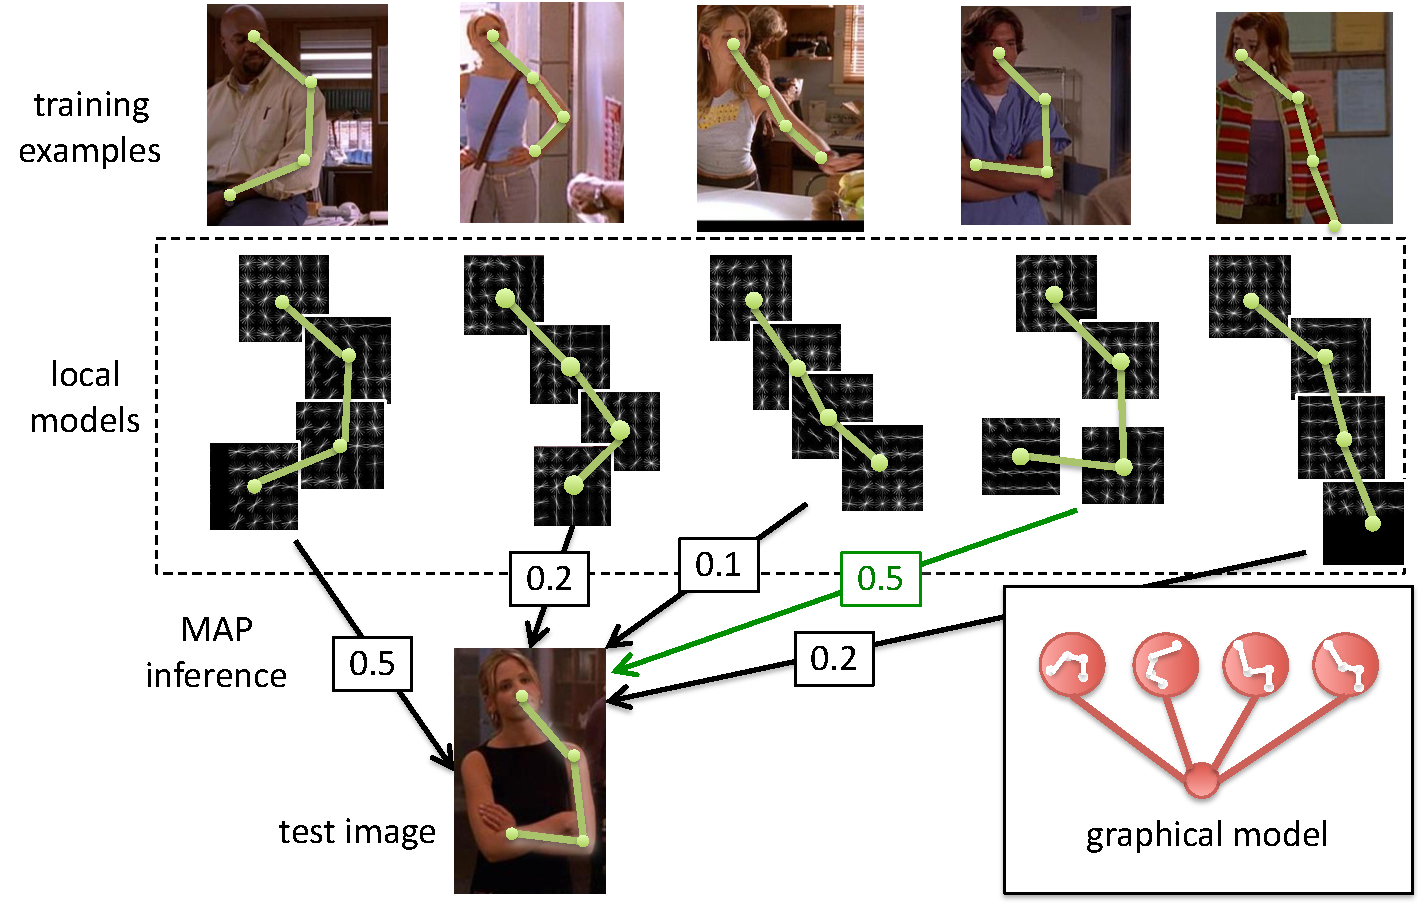
\includegraphics[width=0.99\linewidth]{figs/llps-inference.pdf}
\caption[LLPS inference.]{\label{fig:llps-inference} An illustration of the 
inference process.  Each training example defines a local neighborhood model.  
Each model is run in parallel on a test image, and the argmax prediction is 
taken as a guess. Inset: the graphical model structure.}
\end{figure}

\subsection{Image-adaptive pose priors and a non-parametric perspective}
One important perspective of the above is as a pose {\em switching model}, 
popular in speech synthesis \citep{rosti2003switching}.  In this setting, $z$ 
can be thought of as a switch which chooses between different appearance and 
pose priors.  The particular instantiation of $z$ depends on the image content.  
This is related to another, locally-linear method called Adaptive Pictorial 
Structures (APS) \citet{sapp2010}.  In this work, the pose prior terms 
$\phi_{ij}$ were adjusted based on a kernel-weighted sum of exemplar 
similarities to the image.  \LLPS, on the other hand, forces a discrete choice 
from a dictionary of pose priors, and this procedure is learned 
discriminatively.  From a more practical standpoint, APS relied on very costly 
and heuristic nearest-neighbor computation.  It searched densely through a 
large number of deformations to handle articulation, rather than making use of 
have a decomposable distance.  Each submodel of \LLPS can be thought of as a 
decomposable similarity function, learned discriminatively to separate true 
poses from bad locally, as we will see next.

\section{Learning}\label{sec:llps-learning}

During training, we have access to a training set of images with labeled poses 
$S = \{(x^{t},y^{t})\}_{t=1}^T$.  As described, we choose to model a local 
neighborhood in pose and appearance centered around each training example.  
This allows us to capture fine variations of appearance from pose, clothing, 
lighting, etcetera using a single linear model.

We define a neighborhood set function which maps an image and corresponding 
human pose to a set of indices of ``close'' training samples: $t \in 
\mathcal{N}((x,y))$ means that training sample $t$ is somehow ``close'' to 
$(x,y)$ in appearance and pose.  We will also overload notation to say the 
$\mathcal{N}(t)$ refers to the neighborhood of training sample $t$.  The 
specifics of $\mathcal{N}(\cdot)$ which formalize the notions of closeness in 
pose and appearance are detailed in \secref{nbhd}.

The key idea of learning is that we want to fit parameters so that each local 
model scores higher than other models that are not part of its local 
neighborhood, on the correct pose configuration.  For submodel $m$ centered 
about training sample $(x^m,y^m)$, we would like the large-margin constraints:
\begin{align}
s^m(x^t,y^t) \geq 1 + s^{m}(x^t,y), \label{eq:c1}\\
s^m(x^t,y^t) \geq 1 + s^{m'}(x^t,y),\label{eq:c2}\\
\forall y \in \mathcal{Y}\setminus \{y^t\},~\forall t \in 
\mathcal{N}(m),~\forall m' \notin \mathcal{N}(m) \nonumber
\end{align}
In words,~\equref{c1} states that the score of the true configuration for local 
model $m$ must be higher than $m$'s score for any other (wrong) configuration 
in example $t$.  \equref{c2} states that the score of the true configuration 
for $m$ must also be higher than any score a ``stranger'' model $m' \notin 
\mathcal{N}(m)$ has for any pose configuration in example $t$.  Adding slack 
and regularization on the parameters, we get a convex, large-margin structured 
loss jointly over all $m$ local models

\begin{align}\label{eq:full-learn}
\min_{\{w^m\}, \{\xi_{m,t}\}}& \;\; \sum_{m=1}^M ||w^m||_2^2 + C \sum_{m=1}^M 
\sum_{t \in \mathcal{N}(m)} \left[ \xi_{m,t} + \sum_{m' \notin \mathcal{N}(m)} 
\xi'_{m',t} \right] \\
\text{\bf{subject to:} }
&s^m(x^t,y^t) \geq 1 + s^{m}(x^t,y) - \xi_{m,t}\\
&s^m(x^t,y^t) \geq 1 + s^{m'}(x^t,y) - \xi'_{m',t}\\
&\forall y \in \mathcal{Y}\setminus \{y^t\}, \forall m \in [1,M], \forall t \in 
\mathcal{N}(m), \forall m' \notin \mathcal{N}(m) \nonumber \end{align}

Note that there is in practice significant overlap in neighborhood sets rather than disjoint partitions.  This gives a smoothly varying description of pose space.

\subsection{Decomposable approximate learning}
The learning objective in~\equref{full-learn} couples all models together to 
train them jointly.  While this has attractive properties, it is unwieldy for 
large training sets.  We now propose a series of modifications to the form of 
the model and~\equref{full-learn} to significantly simplify and parallelize 
training.

\mypar{A simpler pairwise cost:}\label{sec:boxdist}
Traditionally, the pairwise cost in PS models has been a simple geometric 
displacement cost: $f_{ij}(x,y_i,y_j) = d(y_i - y_j - \delta_{ij})$, where 
$\delta_{ij}$ is the mean pixel displacement vector between parts $i$ and $j$, 
and $d(\cdot)$ is either a quadratic penalty~\citep{felz05} or a binning 
function~\citep{devacrf}.  These restricted forms of $d(\cdot)$ allow for fast 
inference message passing techniques via convolution or distance transforms.  
We use instead a uniform {\em box deformation cost} defined by 
$f_{ij}(x,y_i,y_j) = 0$ when $|y_i - y_j - \delta_ij| < b$, and $-\infty$ 
otherwise, where $b$ specifies the size of the box in which, given $y_j$, $y_i$ 
is free to deviate from $\delta_{ij}$ in pixel units.  This yields a new form 
for our local model \begin{align}\label{eq:boxdist}
s^m(x,y) = 
\begin{cases}
 \sum_i \w^m_i \cdot \f_i(x,y_i), & |y_i - y_j - \delta_{ij}| < b,\;\; \forall 
(i,j) \in \mathcal{E} \\
 -\infty & \text{otherwise}
 \end{cases}
\end{align}

This formulation has attractive properties: (1) It leads to even faster inference than a quadratic stretching cost, using a 2D min transform instead of a distance transform, (2) less parameters to learn in each local neighborhood.

\mypar{Decoupling local models:} Next, we drop the constraints
$$s^m(x^t,y^t) \geq 1 + s^{m'}(x^t,y), \forall m, \forall m'\notin 
\mathcal{N}(m),\forall t$$ which decouples model $m$'s parameters from all 
other models $m'$.  Model $m$ no longer has to score the correct configuration 
$y^t$ higher than other models' beliefs in the correct configuration.  Instead, 
it only has to score the correct configuration higher than the exponentially 
many incorrect configurations in its local neighborhood of training images.  
This is equivalent to training a single PS model on a subset of the training 
data, independent of other models trained on other, overlapping subsets of the 
training data.  The inherent problem with this is that now different local 
model scores may not be comparable.  We address this with a calibration step 
described in~\secref{calib}.

\mypar{Psuedolikelihood} A final approximation is to assume, for training, that the structured functions $s^m(x,y)$ decompose into independent cliques, and can thus be trained independently.  That is,
$$ s^m(x,y) = \sum_{i} s^m(x,y_i | y_{\mathcal{E}(i)}) $$ 
where $\mathcal{E}(i) = \{j \;|\; (i,j) \in \mathcal{E}\}$.  This is a common 
trick that greatly simplifies structured learning, at the cost of approximation 
error.  Combined with the pairwise cost described in~\equref{boxdist}, this 
amounts to
$$s^m(x,y_i| y_{\mathcal{E}(i)}) = 
\begin{cases}
 \w^m_i \cdot \f_i(x,y_i), & |y_i - y_j - \delta_{ij}| < b,\;\; \forall j \in 
\mathcal{E}(i) \\
 -\infty & \text{otherwise}
\end{cases}
$$
which means we can learn parameters $\w_i^m$ separately for each part $i$ in 
each local model $m$.

In summary, by using a box deformation cost, decoupling the local models and using pseudolikelihood, we train part detectors individually.  The structured SVM learning objective for each part $i$ in each model $m$ is now:

\begin{align}
\min_{\w_i^m}&~||\w_i^m||_2^2 + C \sum_{t} \xi_t\\
\text{subject to: }
& \w_i^m \cdot \f_i(x^t,y_i^t) \geq 1+\w_i^m \cdot \f_i(x^t,y_i)-\xi_t 
\nonumber \\
& \w_i^m \cdot \f_i(x^t,y_i^t) \geq 1+\w_i^m \cdot \f_i(x^{t'},y_i)-\xi_t 
\nonumber \\
&\forall y_i \in \mathcal{Y}_i\setminus \{y_i^t\}, \forall t \in 
\mathcal{N}(m), \forall t' \notin \mathcal{N}(m) \nonumber
\end{align}
We can optimize this using an off-the-shelf standard binary SVM solver.  We 
handle the enormous number of constraints---$O(M \cdot |\mathcal{Y}_i|)$, the 
number of pixel locations in our dataset---by employing a cutting plane method, 
which starts from a random sampling of constraints, and iteratively finds 
violated constraints by mining for false positives, then re-optimizing.

	

\section{Modeling human pose with \LLPS}
In~\secref{llps-model} and~\secref{llps-learning}, we detailed a general 
learning and inference framework for local linear structured models, with 
overlapping and decomposable neighborhood structure.  We now fill in necessary 
details on the graph structure, neighborhood function, and features to describe 
how we apply this model to human pose estimation.
\subsection{Local graph structure}
In order to effectively use training data, we model only one side of a human--- 
the nose, left shoulder, left elbow and left wrist. This allows us to re-use 
training data for the left and right sides by horizontal mirroring, and also 
makes inference faster since we have a simple chain graph connecting each 
joint.  We also insert midpoint nodes into the graph between the semantic 
joints---between the nose and shoulder  (capturing neck curvature), the upper 
arm, and the forearm, similar to~\citet{deva2011}, and thus have $n=7$ parts in 
each local linear structured model.

The decision to split the modeling into sides is also justified empirically.  
Localization accuracy for detecting the torso and head of a person in pose
datasets is near-perfect, thus there is virtually no useful signal for the left 
side of a person to send to the right side through the torso and head, 
regarding beliefs of where parts should go.  In other words, variables on the 
left and right side of the person are d-separated given the torso and head 
variables, which are observed almost deterministically.

\subsection{Local Neighborhoods}\label{sec:nbhd}

As laid out in~\secref{llps-learning}, we define a neighborhood function 
$\mathcal{N}(x,y)$ which takes as input the appearance $x$ and human pose $y$ 
and returns a set of training example indices which are considered part of the 
neighborhood of example $(x,y)$.  We allow our neighborhood function to 
decompose at the level of parts, so that we can mix and match training examples 
when we train models for different joints.  For example, when learning 
parameters centered around example $t$, a different set of other examples may 
be used to train the elbow than are used to train the shoulder parameters.  We 
define our part-based neighborhood as follows, leveraging both appearance and 
geometry:

\mypar{Geometric neighborhood $\mathcal{N}_{geom}(y_i)$:} Around a joint $y_i$, 
we consider two angles and two limb lengths which we use to define our 
geometric neighborhood: the angle that limb $y_i$,$y_{i+1}$ makes with the 
horizontal axis, the inner angle between limbs $y_{i-1}$,$y_i$ and 
$y_{i}$,$y_{i+1}$, and the Euclidean length of limbs $y_{i-1}$,$y_i$ and 
$y_{i}$,$y_{i+1}$.  Stacking these $4$ geometric features into a vector $g_i$, 
we define our geometric neighborhood as $$ \mathcal{N}_{geom}(y_i) = \{\; t 
\text{ s.t. } |g_{ij} - g^t_{ij}| < \tau_j \text{ for $j=1...4$}\;\},$$ 
thresholding on differences of angles and limbs between the example center 
$y_i$ and all other examples $y_i^t$.  In practice we set $\tau_j$ to be a 
tolerance of $5^\circ$ for the two angles, and a tolerance of 6\% of the height 
of a detected upper body for the limb length (more intuitively, approximately 
the palm size of a human hand).


\mypar{Appearance neighborhood $\mathcal{N}_{app}(x,y_i)$:}  While there are 
many examples that are pose similar, we really wish to fit model parameters for 
a set of examples that {\em appears} similar, \eg, to avoid trying to model
different clothing or body types with one linear model.  In light of this, we 
consider a patch centered around joint $y_i$, represented as a HoG descriptor 
vector $h_i$.  We measure the similarity to other examples' HoG descriptor 
patches via normalized cross-correlation, and threshold to obtain our 
appearance neighborhood definition: $$  \mathcal{N}_{app}(x,y_i) = \{\; t 
\text{ s.t. } \frac{h_i}{||h_i||} \cdot \frac{h_i^t}{||h_i^t||} < \tau_h 
\;\},$$ where in practice we set $\tau_h = 0.2$ (normalized cross-correlation's 
range is $[-1,1]$).
Finally, we combine our appearance and geometry neighborhood definitions to 
obtain our neighborhood function $\mathcal{N}(x,y_i) = \mathcal{N}_{geom}(y_i) 
\cap \mathcal{N}_{app}(x,y_i).$

\subsection{Inter-Model Calibration}\label{sec:calib}  As described 
in~\secref{llps-learning}, we decouple the training of our local models, which 
allows us to efficiently train models in parallel.  The downside of this is 
that the bias and variance of the output of each model might vary greatly.  One 
very overconfident local model may always dominate the prediction step.  The 
problem of combining separately-trained models is also an issue in other recent 
works---\citet{johnson11} uses multinomial logistic regression on validation 
data to predict which of 16 PS models to believe per test example, and
Exemplar-SVM~\citep{esvm}, lacking validation data, estimates posterior 
probabilities from already-seen training data. In our implementation, we 
perform inference for each local model on every training example---this data 
was seen during pseudo-likelihood training, but not in full model inference.  
We then estimate a linear scale and offset to map the range of scores of each 
local model on the training set to $[0,1]$.  \\
\mypar{Mode selection:} In an additional step, we also remove redundant or 
malevolent models---ones whose addition to the set of local models hurts 
performance.  On training data, after calibration, we start with an empty set 
of models, and then iteratively greedily choose to add a new local model that 
increases the accuracy of the inlier set.  If we consider each local model as a 
basis, this is a form of basis pursuit.  In practice this results in a 
significantly smaller set of local models at test time, which speeds up 
inference. Details are in~\secref{experiments}.  

